\chapter{Ievads}
Jebkāda veida objektu atpazīšana, neatkarīgi no tā vai tās ir galvas, cilvēki vai jebkāds cits objekts, ir svarīgs uzdevums dažādām datorredzes problēmām. Sejas atpazīšanas problēmas ir zināmas jau diezgan ilgu laiku, taču cilvēku atpazīšana dažādos kameru leņķos, pie dažādām izšķirtspējām, pie dažādiem apgaismojumiem, dažādām cilvēku pozām vai cilvēku atpazīšana attēlos, kuri ir pārpildīti ar cilvēkiem joprojām ir sarežģīts uzdevums.

Autors pētījumā plāno izpētīt metodes, lai varētu novērot cilvēku plūsmu pilsētu objektos, kuri ir nesen izveidoti vai ir nesen tikuši atjaunoti vai remontēti, lai noteiktu ceļu, velosipēdu brauktuvju vai pastaigu taku nolietojumu. Rezultātā tiks iegūta sistēma, kas uzticami varētu veikt cilvēku skaitīšanu video ierakstos vai arī tiešsaistes straumē izmantojot konvolūciju neironu tīklus. Tālāk šādu sistēmu būtu iespējams viegli modificēt, lai to pielietotu objektu skaitīšanai citās nozarēs, piemēram, bioloģijā (šūnu skaitīšana) vai automašīnu skaitīšana.

Tā kā cilvēku detektēšana un sekošana ir sarežģīts process vidē ar augstu cilvēku blīvumu, vairāki aktuālie risinājumi ir balstīti uz regresiju \cite{chen2012feature,chen2013cumulative}. Šo metožu mērķis ir iemācīties sakarību starp zema līmeņa īpašībām attēlos un cilvēku skaitu. Diemžēl, šīs metodes darbosies tikai ainās, kurās tās ir apmācītas. Tas nozīmē, ka šāds cilvēku skaitīšanas modelis katrai ainai ir jāapmāca atsevišķi.

Citas uz konvolūcijas neironu tīkliem balstītas metodes izmanto daudz līmeņu arhitektūras \cite{zhang2016single,onoro2016towards}. Šīs metodes uzrāda labus rezultātus augsta blīvuma, sarežģītās ainās, taču šīs metodes mēdz kļūdīties attēlos ar ļoti mazu pūļa blīvumu, vai ļoti ļoti augstu pūļa blīvumu. Šo problēmu var risināt izmantojot ainu kontekstuālo informāciju. Vairāki eksistējošie pētījumi, kuros izmanto semantisko segmentāciju, ainu parsēšanu un vizuālās īpašības demonstrē, ka kontekstuālās informācijas izmantošana nodrošina nozīmīgus uzlabojumus rezultātos. Tas nozīmē, ka kontekstuālās informācijas izmantošana var palīdzēt apmācības procesā un rezultātā ļaus iegūt precīzāku cilvēku skaita novērojumu \cite{sindagi2017generating}. 

Šī darba nolūkos tiks izmantota "tiešā" objektu skaitīšana, kur katrā ainā tiks meklētas visas cilvēku sejas un tās tiks saskaitītas, kopējo attēla kontekstu neņemot vērā.

Šī darba nolūkos, autors izvirzīja mērķi izstrādāt risinājumu, kas veic cilvēku plūsmas analīzi, pielietojot konvolūcijas tīklu un sekošanas algoritmu analīzi. Lai sasniegtu darba mērķi, ir nepieciešams veikt sekojošus uzdevumus:
\begin{itemize}
	\item Iepazīties ar plūsmas analīzes metodoloģiju, veikt literatūras izpēti;	
	\item Salīdzināt dažādas konvolūcijas neironu tīklu arhitektūras un objektu detektēšanas algoritmus;
	\item Salīdzināt dažādus sekošanas algoritmus;
	\item Izstrādāt risinājumu, kas veic objektu detektēšanu un sekošanu šiem objektiem video kadros;
	\item Pārbaudīt izveidotā risinājuma veiktspēju ar dažādiem video fragmentiem.	
\end{itemize}

Šis darbs sastāv no 5 nodaļām. Pirmajā nodaļā ir veikts ieskats darba aktualitātē, uzskaitīti darba mērķi, uzdevumi. Papildus ir aprakstīts  mašīnmācīšanās pamatjēdziens un kas ir datorredze.

Otrajā nodaļā ir veikts literatūras apskats par klasiskajiem mašīnmācīšanās algoritmiem. Ir izpētīti konvolūcijas neironu tīkli, aprakstīta to struktūra, kādi slāņi parasti sastāda konvolūcijas neironu tīklu, kādas ir populārākās arhitektūras. Aprakstīts kādus ietvarus un programmatūru
var izmantot darbam ar konvolūcijas neironu tīkliem un kā apmācīt šos tīklus. Tika veikta literatūras izpēte par aktuālajiem cilvēku plūsmas analīzes risinājumiem, šim darbam aktuālajiem objektu detektēšanas un sekošanas algoritmiem.

Trešajā nodaļā ir aprakstīta darbā izvēlētā plūsmas analīzes implementācija. Aprakstīts kā sagatavot datus, lai veiktu apmācītu \textit{YOLO} un \textit{SSD} objektu detektēšanas sistēmas, kā tika mainīta konfigurācija, lai apmācītu konvolūcijas neironu tīklus minētājām objektu detektēšanas sistēmām un kā vienā risinājumā tika savienoti objektu detektēšanas algoritmi ar sekošanas algoritmiem.

Ceturtajā nodaļā ir aprakstīti izveidotā risinājuma rezultāti, cik labi dažādi sekošanas algoritmi spēja sekot detektētajiem objektiem.

Piektajā nodaļā ir aprakstīti pēc literatūras izpētes un risinājuma implementācijas izvirzītie secinājumi un priekšlikumi.
\newpage
\section{Mašīnmācīšanās pamatjēdziens}
Mašīnmācīšanās algoritmi ir kļuvuši par neatņemamu sastāvdaļu programmatūras izstrādātājiem un kompānijām, kas savas aplikācijas grib padarīt "gudras". Lai arī cik, mūsdienās, šis jēdziens ir kļuvis populārs, oficiāla mašīnmācīšanās definīcija nav noteikta. Visvienkāršākais mašīnmācīšanās pielietojums ir apstrādāt datus, mācīties no tiem un no iegūtajiem rezultātiem pieņemt lēmumus vai veikt minējumus reālās pasaules problēmu risināšanai. Tā vietā, lai manuāli veidotu programmatūras risinājumus, kas veic kādu uzdevumu, tiek apmācīti datori vai citas ierīces, izmantojot lielus datu apjomus. 
Pasaulē ir daudz un dažādi mašīnmācīšanās algoritmi un katru dienu tiek publicēti simtiem jaunu algoritmu. Tos var sagrupēt pēc apmācības veida (vadītā apmācība (\textit{supervised learning}), nevadītā apmācība (\textit{unsupervised learning}), pusvadītā apmācība (\textit{semi-supervised learning})) kā arī pēc formas vai funkcijas līdzībām (klasifikācija, regresija, lēmumu koki (\textit{decision trees}), klasterēšana (\textit{clustering}), dziļā mašīnmācīšanās (\textit{deep learning})). Neatkarīgi no apmācības veida vai pielietojuma, visas mašīnmācīšanās algoritmu kombinācijas sastāv no klasifikatoriem (atbalsta vektora mašīna, lēmuma koki, neironu tīkli), vērtēšanas funkcijām (varbūtības funkcijas, robežfunkcijas, izmaksu funkcija) un optimizācijas funkcijām (mantkārīgā meklēšana, nepārtrauktās optimizācijas metodes (\textit{continuous optimization})). Izmantojot šīs sastāvdaļas, mašīnmācīšanās algoritmu pamata mērķis ir būt spējīgam funkcionēt ne tikai ar apmācībā piedāvātajiem datiem, bet arī spēt darboties ar datiem, ar kuriem algoritms nav saskāries. Atkarībā no veicamā uzdevuma, ir dažādi veidi kā panākt, lai datori vai jebkura cita ierīce mācās, sākot ar visparastākajiem lēmumu kokiem, beidzot ar ģenētiskajiem algoritmiem un mākslīgajiem neironu tīkliem. 


\section{Datorredze}
Datorredze (no angļu val. \textit{computer vision}) ir datorzinātņu nozare, kuras mērķis ir ļaut datoriem redzēt un veikt tādus pašus uzdevumus kā cilvēki veiktu ar acīm un darīt to tikpat efektīvi. Redzes nodrošināšana datoriem nozīmē dot tiem spēju identificēt un apstrādāt attēlus līdzīgi kā to spēj darīt cilvēki. Tas ir kā nodot cilvēku inteliģenci un instinktus datoram. Datorredzes sistēmas parasti iedala trīs komponentēs:
\begin{itemize}
	\item Attēla iegūšana;
	\item Attēla apstrāde;
	\item Attēla analīze;
\end{itemize}
Līdzīgi kā cilvēku pasaules izpratne balstās uz spēju pieņemt lēmumus ņemot vērā redzēto, piedāvājot datoriem šādu vizuālu izpratni, tiem būtu iespējams pieņemt patstāvīgus lēmumus.

\begin{figure}[h]%
	\centering
	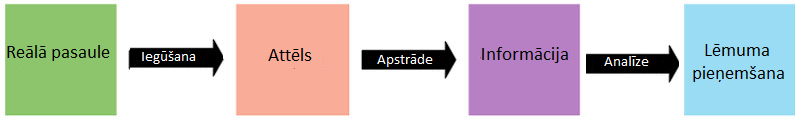
\includegraphics[height=2cm]{images/computervision1.png} %
	\caption{Datorredzes pamatprincips}%
	\label{fig:example}%
\end{figure}

Attēlu iegūšana ir process kurā reālās pasaules notikumi tiek pārveidoti bināros datos, kurus interpretē kā digitālus attēlus vai kā daļu no video fragmenta. 

Attēlu apstrāde ir iegūto attēlu zema līmeņa apstrāde. Pirmajā solī iegūtajiem binārajiem datiem pielieto algoritmus, kas norāda uz attēla daļām, kas satur zema līmeņa informāciju. Šādu informāciju var izšķirt pēc jebkādiem ģeometriskiem elementiem, kas sastāda attēlu, piemēram, punkti attēlā, attēla malas vai segmenti. Zema līmeņa attēlu apstrādes algoritmi ir malu detektēšana, segmentācijas algoritmi, klasifikācija, īpašību detektēšana.
\begin{figure}[h]%
	\centering
	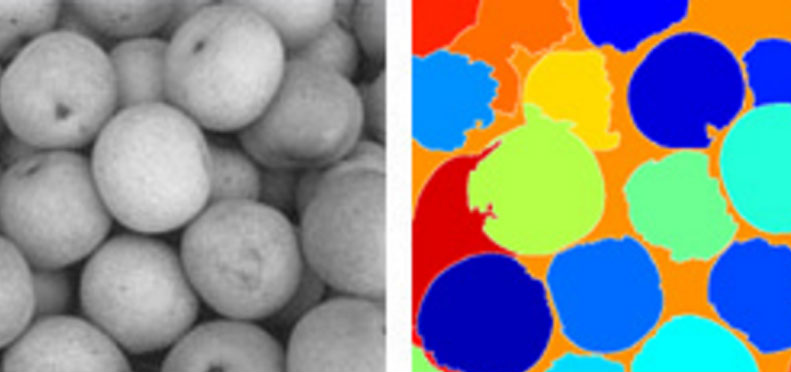
\includegraphics[height=3cm]{images/computervision2.png} %
	\caption{Ābolu segmentācija attēlā \cite{compv1}}%
	\label{fig:example}%
\end{figure} 

Pēdējā datorredzes sistēmu komponente ir attēlu analīzes solis, kurā notiks attēla analīze un pēc šī soļa datorredzes sistēmai būs iespējams pieņemt lēmumu un izvadē to atgriezt. Attēlu analīzes solī tiek pielietoti augsta līmeņa algoritmi, ņemot vērā gan attēla apstrādes solī iegūto zema līmeņa informāciju, gan pašu attēlu. Piemēri kur var izmantot šādu augsta līmeņa attēlu analīzi ir trīsdimensiju ainu atveidošana, objektu atpazīšana, objektu sekošana, cilvēku plūsmas analīze.
\begin{figure}[h]%
	\centering
	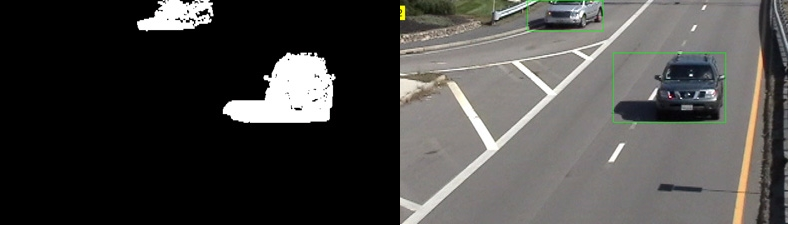
\includegraphics[height=4cm]{images/computervision3.png} %
	\caption{Objektu detektēšana pēc segmentācijas pielietošanas \cite{compv2}}%
	\label{fig:example}%
\end{figure} 

Izstrādājot datorredzes sistēmas, pētnieki saskaras ar dažādām problēmām un izaicinājumiem. Parasti šīs problēmas ir atkarīgas no datu kvalitātes, sistēmas pielietojuma un apkārtējās pasaules ietekmes uz datiem un aparatūru. Datorredzes pētnieki izstrādā risinājumus, lai padarītu datorredzes algoritmus stabilākus un efektīvākus sarežģītos uzstādījumos: nekvalitatīvi vai trokšņaini dati, reālā laika apstrāde un ierobežota skaitļošanas jauda. Mūsdienās, lai risinātu šīs problēmas, tiek savienoti mašīnmācīšanās risinājumi ar datorredzes risinājumiem.

Klasiskie datorredzes algoritmi ir smalki pētīti un optimizēti, lai iegūtu labāko veiktspēju un lai tie efektīvi izmantotu datora skaitļošanas resursus, savukārt mašīnmācīšanās algoritmi piedāvā precīzākus un vispusīgākus risinājumus, taču prasa lielus skaitļošanas resursus. Ņemot vērā iepriekš minēto, mūsdienu pētījumos ir populāri risinājumi, kas apvieno standarta datorredzes algoritmus un mašīnmācīšanās risinājumus. Labs piemērs abu šo nozaru apvienošanā ir kustīgu objektu meklēšana video fragmentos. Lai iegūtu augstāku precizitāti un taupītu skaitļošanas resursus ir iespējams attēla apstrādi veikt ar datorredzes algoritmiem un attēla analīzi (klasifikāciju, lokalizāciju, sekošanu) veikt ar neironu tīkliem.



